\chapter*{Задание}

В информационный центр приходят клиенты через интервалы времени $10\pm2$ минуты. Если все три, имеющихся оператора, заняты, клиенту отказывают в обслуживании. Операторы имеют разную производительность. И могут обеспечивать обслуживание среднего запроса за $20\pm5$, $40\pm10$, $40\pm20$ минут. Клиенты стремятся занять свободного оператора с максимальной производительностью. Полученные запросы сдаются в приемные накопители, откуда они выбираются для обработки. На 1-ый компьютер запросы от 2-ого и 1-ого оператора. На 2-ой компьютер от 3-его оператора. Время обработки на 1-ом и 2-ом компьютере равны соответственно 15 и 30 минутам.

Смоделировать процесс обработки 300 запросов.

\begin{figure}[h]
	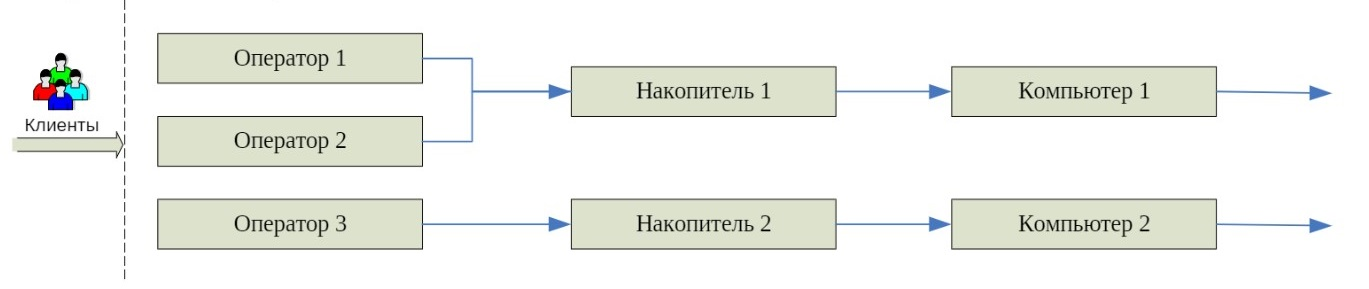
\includegraphics[width=1\linewidth]{inc/img/schema1.jpg}
	\caption{Схема модели}
	\label{s1}
\end{figure}